
% ============================================================
% Schöne, aber schnelle und weiterbearbeitbare Kochbuch-Praeambel
% ============================================================
\usepackage[T1]{fontenc}
\usepackage[utf8]{inputenc}
\usepackage[ngerman]{babel}
\usepackage{microtype}
\usepackage{tgpagella}
\usepackage{graphicx}
\usepackage{xcolor}
\usepackage{geometry}
\usepackage{etoc}
\usepackage{etoolbox}
\usepackage{multicol}
\usepackage{totcount}
\usepackage{makeidx}
\usepackage{nicefrac}
\usepackage{titlesec}
\usepackage{xurl}
\usepackage{hyperref}
\usepackage[nowarnings]{xcookybooky}

\makeindex
\newtotcounter{recipecount}
\regtotcounter{section}
\AtBeginEnvironment{recipe}{\stepcounter{recipecount}}
\renewcommand{\theHstep}{\arabic{recipecount}.\arabic{step}}

\DeclareRobustCommand{\textcelcius}{\ensuremath{^{\circ}\mathrm{C}}}
\newcommand{\recipesource}[2]{\href{#1}{#2}}

\definecolor{WarmPaper}{HTML}{FBF4E8}
\definecolor{Flour}{HTML}{FFF9EE}
\definecolor{Cream}{HTML}{F0DFC0}
\definecolor{Cocoa}{HTML}{4B2E22}
\definecolor{Tomato}{HTML}{B64B36}
\definecolor{Basil}{HTML}{557A46}
\definecolor{Sage}{HTML}{8B9A6E}
\definecolor{InkGray}{HTML}{3E3832}

\hypersetup{% 
    pdfauthor            = {Adrian Hieber},
    pdftitle             = {Rezeptbuch von Adrian Hieber},
    pdfsubject           = {Rezeptbuch},
    pdfkeywords          = {rezept, rezeptbuch, kochen, vegetarisch, vegan},
    pdfstartview         = {FitV},
    pdfview              = {FitH},
    pdfpagemode          = {UseNone},
    bookmarksopen        = {true},
    colorlinks           = {true},
    linkcolor            = {Cocoa},
    urlcolor             = {Tomato},
    citecolor            = {Cocoa},
    filecolor            = {Cocoa},
}
\urlstyle{same}
\pdfstringdefDisableCommands{%
  \def\step{}%
  \def\lettrine#1#2{#1#2}%
  \def\textcolor#1#2{#2}%
}


% ============================================================
% Schnelles Kochbuch-Design: warm, farbig, editierbar
% ============================================================
\geometry{a4paper, inner=22mm, outer=18mm, top=20mm, bottom=22mm, headheight=16pt, headsep=8mm, footskip=10mm}
\pagecolor{WarmPaper}
\color{InkGray}
\setlength{\parindent}{0pt}
\setlength{\parskip}{0.78em plus 0.25em minus 0.1em}
\setcounter{secnumdepth}{1}
\setcounter{tocdepth}{1}

\setRecipeLengths{%
  pictureheight=5.0cm,
  bigpicturewidth=0.36\textwidth,
  smallpicturewidth=0.26\textwidth,
  introductionwidth=\textwidth,
  preparationwidth=0.59\textwidth,
  ingredientswidth=0.36\textwidth
}
\setRecipeColors{%
  recipename=Tomato,
  intro=InkGray,
  ing=InkGray,
  inghead=Cocoa,
  prep=InkGray,
  prephead=Cocoa,
  suggestion=Cocoa,
  suggestionhead=Tomato,
  separationgraph=Sage,
  hint=InkGray,
  hinthead=Tomato,
  hintline=Tomato,
  numeration=Tomato
}
\setRecipeSizes{%
  recipename=\fontsize{25pt}{29pt},
  intro=\small,
  ing=\small,
  inghead=\large,
  prep=\small,
  prephead=\large,
  suggestion=\small,
  hint=\small,
  hinthead=\large
}
\setRecipenameFont{qpl}{T1}{b}{n}

% Kopf-/Fusszeile
\pagestyle{fancy}
\fancyhf{}
\renewcommand{\headrulewidth}{0pt}
\fancyhead[LE,RO]{\small\color{Cocoa}\rightmark}
\fancyfoot[LE,RO]{\bfseries\color{Tomato}\thepage}
\fancyfoot[C]{\color{Sage}\rule{0.28\textwidth}{0.5pt}\hspace{0.8em}{\color{Tomato}\textbullet}\hspace{0.8em}\rule{0.28\textwidth}{0.5pt}}
\renewcommand{\sectionmark}[1]{\markright{\MakeUppercase{\thesection.\ #1}}}
\renewcommand{\subsectionmark}[1]{}

% Kapitelueberschriften
\titleformat{\section}[display]
  {\bfseries\color{Cocoa}}
  {\Large\color{Tomato}Kapitel \thesection}
  {0.35em}
  {\Huge}
  [{\vspace{0.25em}{\color{Sage}\rule{0.60\textwidth}{1pt}}}]
\titlespacing*{\section}{0pt}{0.4cm}{0.7cm}

\titleformat{\subsection}[block]
  {\bfseries\color{Tomato}}
  {}
  {0pt}
  {}
  [{\vspace{-0.2em}{\color{Sage!70!black}\rule{0.70\textwidth}{0.6pt}}}]
\titlespacing*{\subsection}{0pt}{0.6cm}{0.5cm}

% Kapitel mit einem zweiten, nur im Inhaltsverzeichnis sichtbaren Untertitel.
\DeclareRobustCommand{\cookbooktocsubtitle}[1]{}
\newcommand{\cookbooksection}[2]{%
  \section[{#1\protect\cookbooktocsubtitle{#2}}]{#1}%
}
\pdfstringdefDisableCommands{%
  \def\cookbooktocsubtitle#1{}%
}

% Deckblatt
\newcommand{\cookbooktitlepage}{%
\begin{titlepage}
\thispagestyle{empty}
\pagecolor{WarmPaper}
\vspace*{0.7cm}
\begin{center}
  {\color{Sage}\rule{0.78\textwidth}{1pt}}\\[0.8cm]
  {\bfseries\fontsize{46}{50}\selectfont\color{Cocoa}Adrians Rezeptbuch\par}
  \vspace{0.3cm}
  {\Large\color{Tomato}Eine iterative Sammlung\par}
  \vspace{0.9cm}
  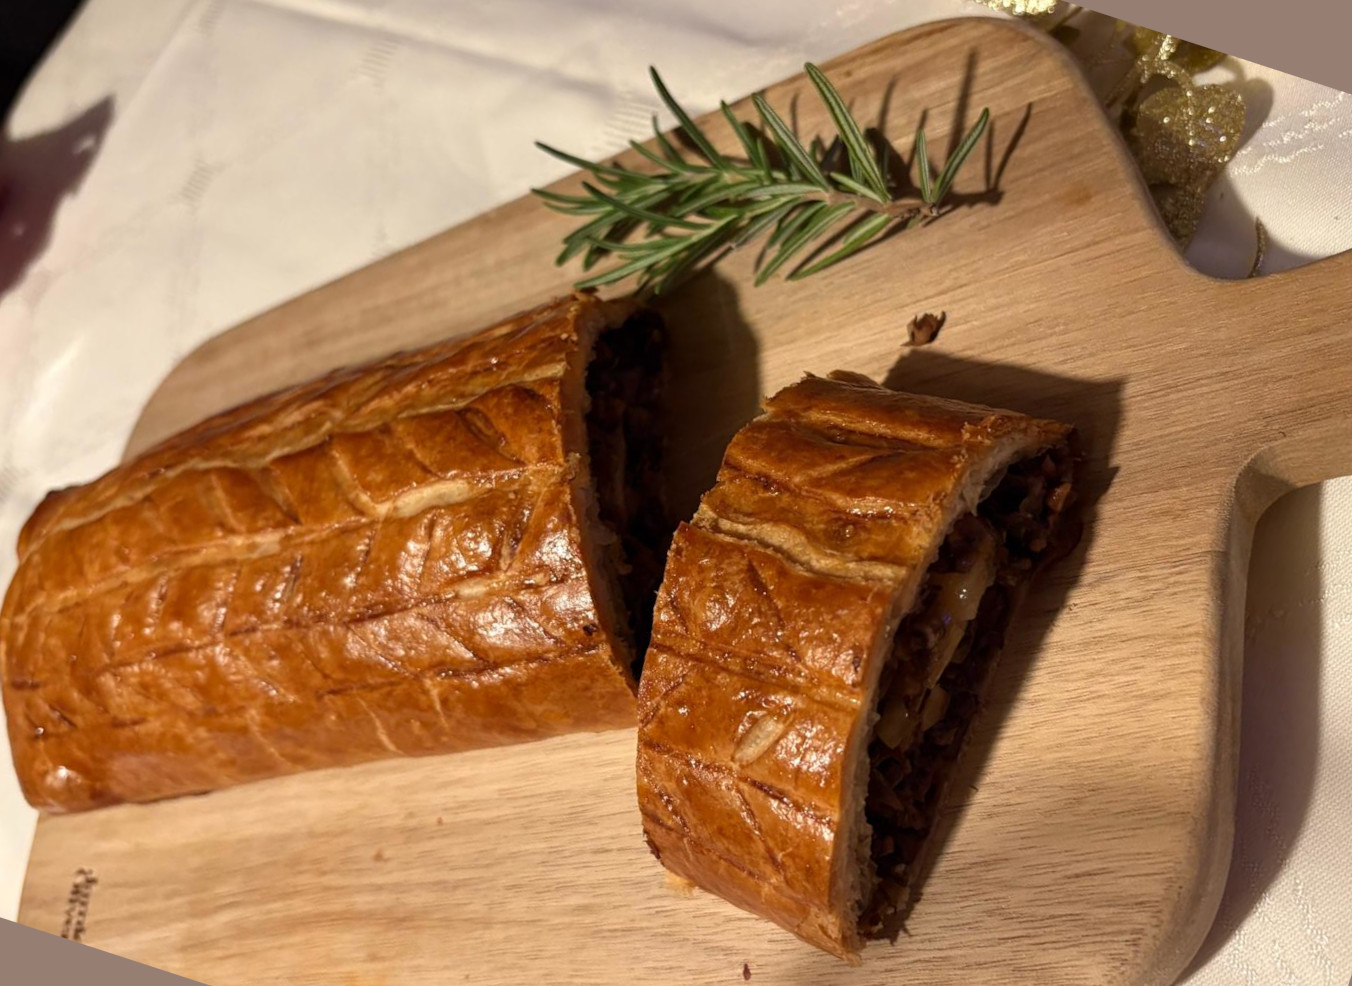
\includegraphics[width=0.80\textwidth,height=0.42\textheight,keepaspectratio]{pic/hauptgericht/07_veggi-beef-wellington-big}
  \vspace{0.8cm}

  \begingroup\setlength{\fboxsep}{10pt}
  \fcolorbox{Sage}{Flour}{\begin{minipage}{0.72\textwidth}
  \small
  Vegetarische und vegane Lieblingsrezepte, Küchenexperimente, Basics und Gerichte, die sich lohnen. Aktuell sind in diesem Projekt \textbf{\total{recipecount}} Rezepte gesammelt.
  \end{minipage}}
  \endgroup

  \vfill
  {\large\bfseries Adrian Hieber}\par
  \href{mailto:adrian.hieber@gmail.com}{adrian.hieber@gmail.com}\par
  \vspace{0.25cm}
  {\today}\par
  \vspace{0.5cm}
  {\color{Sage}\rule{0.78\textwidth}{1pt}}
\end{center}
\end{titlepage}%
}

% Inhaltsverzeichnis-Seite
\makeatletter
\newcommand{\cookbooktocpage}{%
\clearpage
\thispagestyle{empty}
\vspace*{0.5cm}
{\bfseries\fontsize{34}{38}\selectfont\color{Cocoa}Inhalt}\par
\vspace{0.18cm}
{\large\color{Sage}\total{recipecount} Rezepte
  \hspace{0.55em}{\color{Tomato}\textbullet}\hspace{0.55em}
  \total{section} Kapitel}\par
\vspace{0.35cm}
{\color{Tomato}\rule{\textwidth}{1.2pt}}\par
\vspace{0.45cm}
\begingroup
\renewcommand{\cookbooktocsubtitle}[1]{%
  \\[-0.08em]\hspace*{3.25em}{\normalfont\small\color{Sage}##1}%
}
\renewcommand*\l@section[2]{%
  \par\addvspace{0.28em}%
  \noindent
  \begin{minipage}[t]{0.88\linewidth}
    \renewcommand\numberline[1]{%
      \makebox[3.25em][l]{%
        \color{Tomato}\fontsize{16}{18}\selectfont\bfseries
        \ifnum####1<10 0\fi####1%
      }%
    }%
    {\large\bfseries\color{Cocoa}##1}%
  \end{minipage}\hfill
  \begin{minipage}[t]{0.07\linewidth}
    \raggedleft\large\bfseries\color{Tomato}##2
  \end{minipage}\par
}%
\etocsettocstyle{}{}%
\etocsettocdepth{section}%
\tableofcontents%
\endgroup
\clearpage
}
\makeatother

% Zutatenregister: klare Warengruppen, darunter alphabetische Zutaten.
\makeatletter
\fancypagestyle{cookbookindexfirst}{%
  \fancyhf{}%
  \renewcommand{\headrulewidth}{0pt}%
  \fancyfoot[LE,RO]{\bfseries\color{Tomato}\thepage}%
  \fancyfoot[C]{\color{Sage}\rule{0.28\textwidth}{0.5pt}\hspace{0.8em}{\color{Tomato}\textbullet}\hspace{0.8em}\rule{0.28\textwidth}{0.5pt}}%
}
\newif\ifcookbookfirstindexsubitem
\newcommand{\cookbookindexgroup}{%
  \global\cookbookfirstindexsubitemtrue
  \par\addvspace{0.75em}%
  \noindent\bfseries\color{Tomato}%
}
\renewenvironment{theindex}{%
  \clearpage
  \thispagestyle{cookbookindexfirst}%
  \markright{ZUTATENREGISTER}%
  \vspace*{0.25cm}
  {\bfseries\fontsize{31}{35}\selectfont\color{Cocoa}Zutatenregister}\par
  \vspace{0.12cm}
  {\large\color{Sage}Zutaten nach Warengruppen und Seiten}\par
  \vspace{0.3cm}
  {\color{Tomato}\rule{\textwidth}{1.2pt}}\par
  \vspace{0.25cm}
  \setlength{\columnsep}{0.7cm}%
  \setlength{\columnseprule}{0pt}%
  \begin{multicols}{3}
  \footnotesize
  \setlength{\parindent}{0pt}%
  \setlength{\parskip}{0pt}%
  \let\item\cookbookindexgroup
  \renewcommand{\subitem}{%
    \par
    \ifcookbookfirstindexsubitem
      \nobreak\global\cookbookfirstindexsubitemfalse
    \fi
    \hangindent=0.9em\hspace*{0.65em}%
    \normalfont\color{InkGray}%
  }%
  \renewcommand{\subsubitem}{%
    \par\nobreak\hangindent=1.8em\hspace*{1.5em}%
    \normalfont\color{InkGray}%
  }%
  \renewcommand{\indexspace}{\par\vspace{0.35em}}%
}{%
  \end{multicols}
  \clearpage
}
\makeatother

% Schlichte Kapiteltrenner mit Bild; Titel/Untertitel sind in book_schoen.tex editierbar
\newcommand{\chapteropener}[3]{%
\clearpage
\thispagestyle{empty}
\vspace*{1.2cm}
{\color{Sage}\rule{0.66\textwidth}{1pt}}\par\vspace{0.65cm}
{\bfseries\fontsize{38}{43}\selectfont\color{Cocoa}#1\par}
\vspace{0.25cm}
{\Large\color{Tomato}#3\par}
\vspace{0.8cm}
\includegraphics[width=0.92\textwidth,height=0.48\textheight,keepaspectratio]{#2}\par\vspace{0.8cm}
\vfill
{\itshape\color{InkGray}Kochen ist Iteration. Release. Taste. Improve.}\par
\vspace{0.5cm}
{\color{Sage}\rule{0.66\textwidth}{1pt}}
\clearpage
}

% Kleine optische Anpassungen an den Rezeptbausteinen, ohne schwere Boxen
\makeatletter
\renewcommand{\introduction}[1]{%
  \def\xcb@introduction{%
    \begingroup\setlength{\fboxsep}{8pt}%
    \noindent\fcolorbox{Sage}{Flour}{\begin{minipage}{0.96\linewidth}
    {\xcb@fontsize@intro\color{\xcb@color@intro}#1}
    \end{minipage}}%
    \endgroup
  }%
}
\renewcommand{\preparation}[1]{%
  \def\xcb@preparation{%
    {\bfseries\large\color{Cocoa}\xcb@name@prephead}\par\vspace{.15em}
    {\color{Sage}\rule{\linewidth}{.7pt}}\par\vspace{.35em}
    {\xcb@fontsize@prep\color{\xcb@color@prep}#1\par}%
  }%
  \setcounter{step}{0}%
}
\renewcommand{\ingredients}[2][\empty]{%
  \def\xcb@ingredientslines{#1}%
  \def\xcb@ingredients{%
    {\bfseries\large\color{Cocoa}\xcb@name@inghead}\par\vspace{.15em}
    {\color{Sage}\rule{\linewidth}{.7pt}}\par\vspace{.35em}
    {\xcb@fontsize@ing\color{\xcb@color@ing}\begin{tabulary}{\linewidth}{>{\bfseries\color{Tomato}}rL}#2\end{tabulary}}%
  }%
}
\DeclareRobustCommand{\step}{%
  \refstepcounter{step}%
  \lettrine[lines=2,lhang=0.08,loversize=0.04,findent=0.55em,nindent=0em]{{\color{Tomato}\bfseries\thestep}}{}%
}
\makeatother


% \newcommand{\mylocaltableofcontents}{%
%   \vspace{0.5em}
%   \begingroup
%   \setlength{\fboxsep}{8pt}%
%   \noindent\fcolorbox{Sage}{Flour}{\begin{minipage}{0.95\linewidth}
%     \etocsettocstyle{}{}%
%     \etocsettocdepth{subsection}%
%     \localtableofcontents%
%   \end{minipage}}%
%   \endgroup
%   \vspace{0.7em}
% }

\newcommand{\mylocaltableofcontents}{
  \vspace{1em}
  \etocsettocstyle{}{}%
  \etocsettocdepth{subsection}%
  \localtableofcontents%
}

\hbadness=10000
\raggedbottom%
